\documentclass[12pt]{article}
\usepackage{graphicx}
\usepackage{url}

\usepackage{listings}
\usepackage{xcolor}
\lstset { %
   language=C++,
   backgroundcolor=\color{black!5}, % set backgroundcolor
   basicstyle=\footnotesize,% basic font setting
}


\title{Why would you sort when you know where things approximately belong?}
\author{Peter Taraba \footnote{Berkeley, CA 94709}}

\begin{document}

	
	\maketitle
	
	\begin{abstract}
  		We introduce statistical sorting, which has $O(n)$ time complexity on average, and compare it with mainstream C++ std (standard template library) sort, which has on average $O(n \log n)$ time complexity. We show it on three different distributions - uniform, Gauss and an additional one.
	\end{abstract}
	
	\section{Introduction}
	
		Currently, the most popular algorithm for sorting is the quick sort algorithm, which has $O(n \log n)$ time complexity on average \cite{numrec} and in the worst case $O(n^2)$. This publication introduces statistical sorting with $O(n)$ time complexity. In C++, the std::sort() function is implemented using the Intro Sort Algorithm, which combines three standard sorting algorithms: insertion sort, quick sort, and heap sort \cite{cppsort}. On average, they all have $O(n \log n)$ time complexity \cite{wikisort}.
		
		In section 2, we introduce the statistical algorithm, in section 3 we show simple implementation in C++, in section 4 we compare it with C++ std sort, in section 5 we talk about simple parallelization of the statistical algorithm and finally in section 6, we draw conclusions and discuss future work.

	\section{Stat Sort Algorithm}
	
		The simple idea behind statistical sorting is to go through the vector, find its minimum and maximum value (which is $O(n)$), and then split the vector into many tiny ones, which will be sorted either by the same algorithm (in case size of the vector is more than a chosen threshold; for this publication, we chose threshold 10) or by standard sorting algorithms (C++ std sort, etc). For this publication, we chose the number of vectors we split the initial vector of size $s$ as $\sqrt{s}$. This was satisfactory to achieve better time complexity performance ($O(n)$) than other sorting algorithms, which usually have on average $O(n \log n)$ time complexity. We show this on several examples - uniform distribution, Gaussian distribution (\cite{gauss}) as well as one additional distribution. As the implementation of the statistical sorting is very short in C++, instead of describing it in too many details, we provide the entire algorithm in the following section.
		
		
	\section{Stat Sort Algorithm Implementation in C++}
	
	C++ implementation of the basic statistical sorting is as followed:
	
		\begin{lstlisting}
void statsort(vector<double> &vec)
{
   double min, max;

   min = std::numeric_limits<double>::max();
   max = std::numeric_limits<double>::lowest();

   for(long int i=0;i<vec.size();i++)
   {
       if(min>vec[i])
       {
           min = vec[i];
       }
       if(max<vec[i])
       {
           max = vec[i];
       }
   }

   max += 0.0001 * (max-min);

   int memsize = sqrt(vec.size());

   std::vector<double> *myvectors =
   		new std::vector<double>[memsize];

   for(long int i=0;i<vec.size();i++)
   {
       long int where = (int)((vec[i]-min) *
       		(memsize + 0.0) / (max-min));

       myvectors[where].push_back(vec[i]);
   }

   for(long int i=0;i<memsize;i++)
   {
       if(myvectors[i].size()>10)
       {
           statsort(myvectors[i]);
       }
       else
       {
           std::sort (myvectors[i].begin(), myvectors[i].end());
       }
   }

   vec.clear();
   for(long int i=0;i<memsize;i++)
   {
       for(int j=0;j<myvectors[i].size();j++)
       {
           vec.push_back(myvectors[i][j]);
       }
   }
   delete[] myvectors;
}
		\end{lstlisting}
	
	\section{Std Sort vs Stat Sort}
	
		Measured times of std sort and stat sort are in figure \ref{fig1}, as well as theoretical $O(n \log n)$ and $O(n)$ time complexity determined by linear regression and minimum residual.

		\begin{figure}
		\begin{center}
			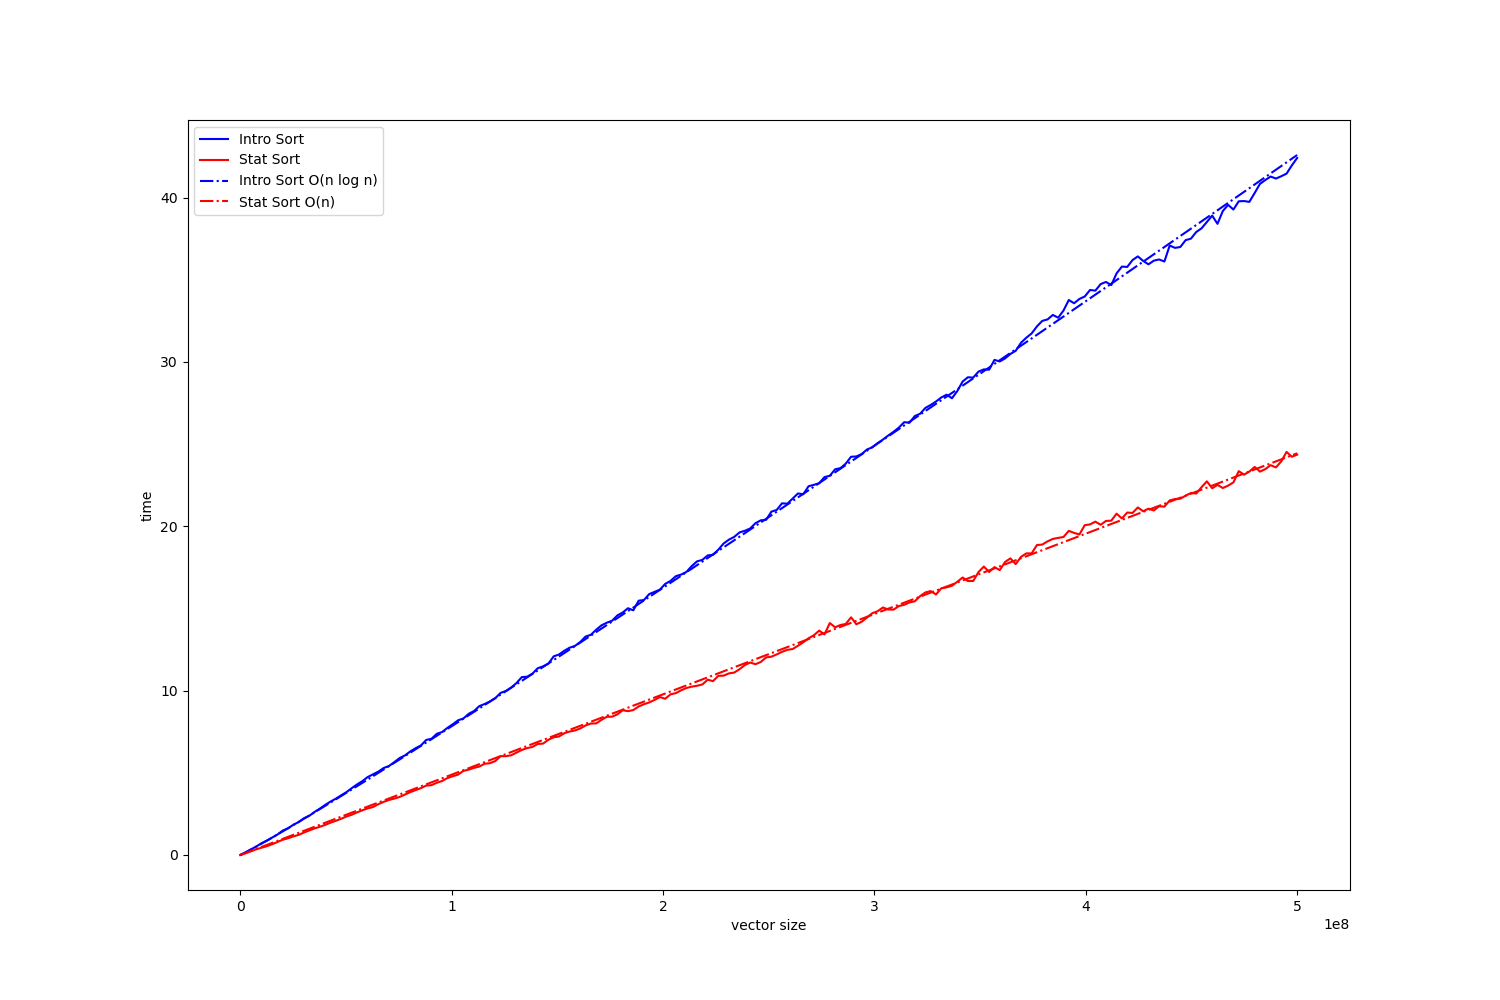
\includegraphics[width=0.7\textwidth]{fig_perf_norm}
		\end{center}
			\caption{C++ std sort (blue) vs C++ stat sort (red) for uniform distribution vector. Full lines are measured times, the dashed blue line is $O(n \log n)$ for C++ std sort, and the dashed red line is $O(n)$ for C++ stat sort determined by residuals from linear regression fit.}
		
		\label{fig1}
		\end{figure}		

		\begin{figure}
		\begin{center}
			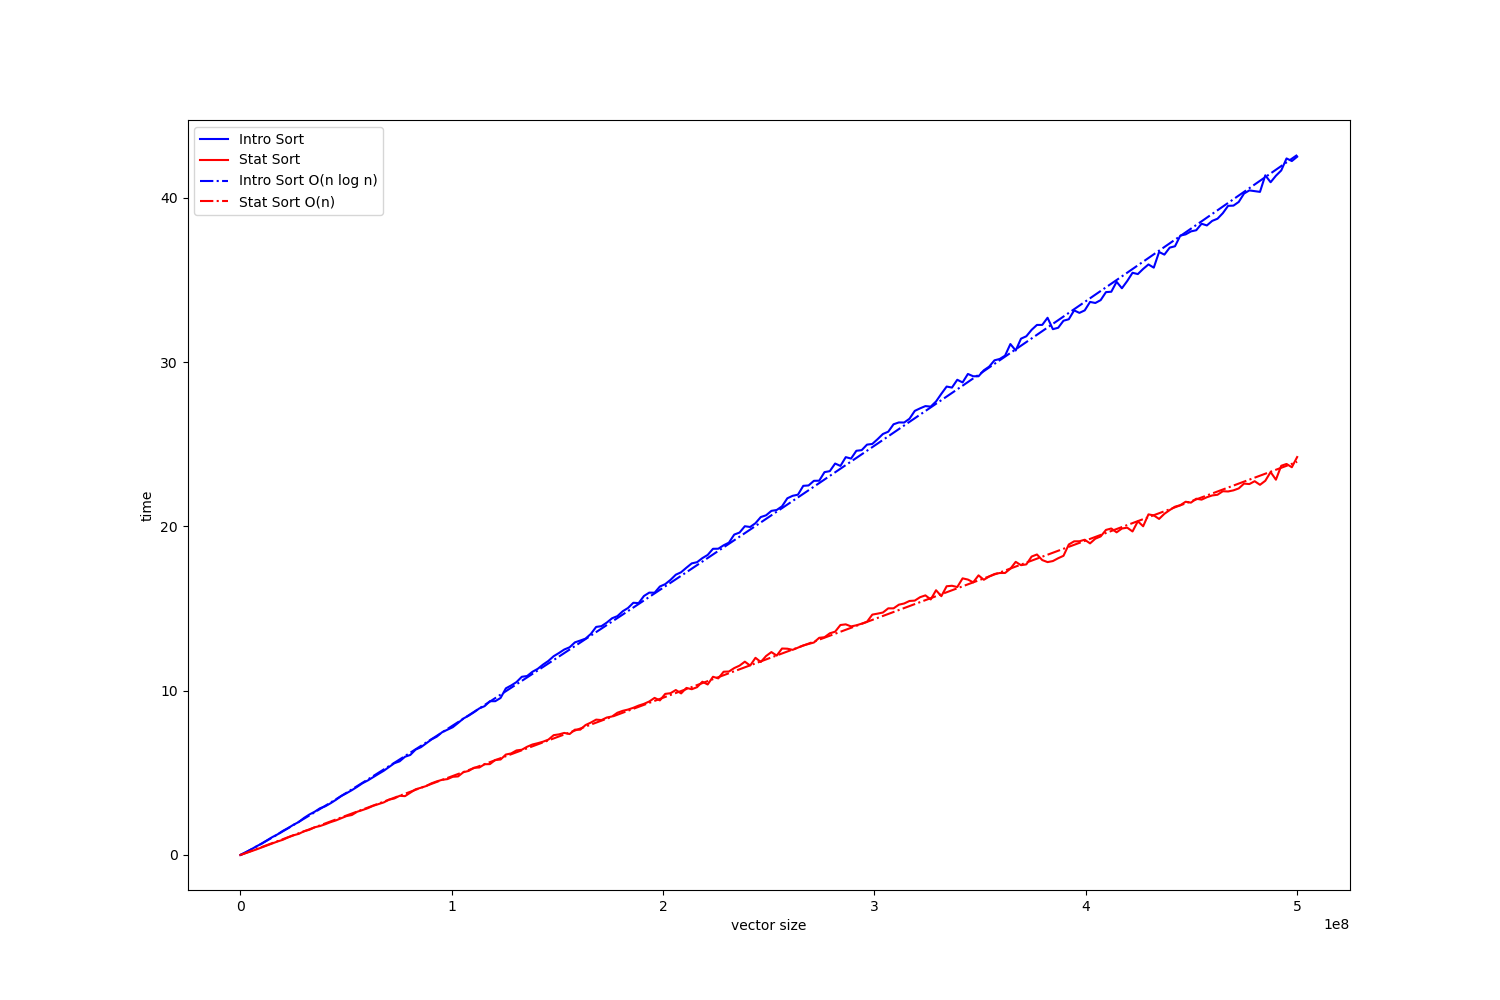
\includegraphics[width=0.7\textwidth]{fig_perf_gauss}
		\end{center}
			\caption{C++ std sort (blue) vs C++ stat sort (red) for Gaussian distribution vector. Full lines are measured times, the dashed blue line is $O(n \log n)$ for C++ std sort, and the dashed red line is $O(n)$ for C++ stat sort determined by residuals from linear regression fit.}
		
		\label{fig2}
		\end{figure}		

		\begin{figure}
		\begin{center}
			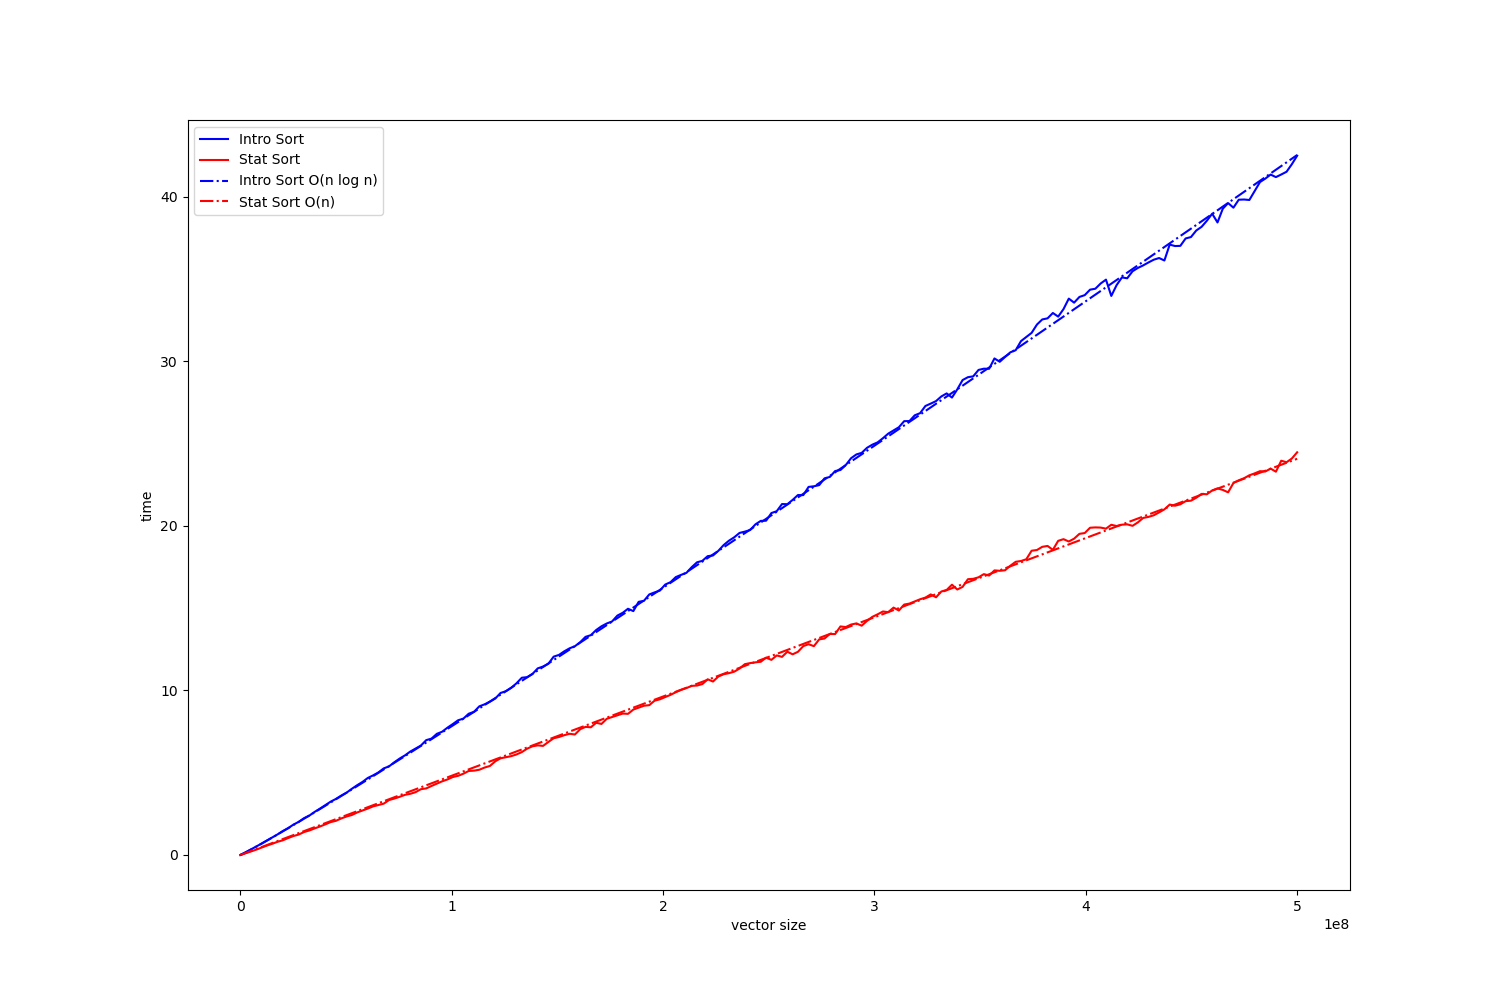
\includegraphics[width=0.7\textwidth]{fig_perf_weird}
		\end{center}
			\caption{C++ std sort (blue) vs C++ stat sort (red) for an additional distribution vector. Full lines are measured times, the dashed blue line is $O(n \log n)$ for C++ std sort, and the dashed red line is $O(n)$ for C++ stat sort determined by residuals from linear regression fit.}
		
		\label{fig3}
		\end{figure}		
		
		\begin{figure}
		\begin{center}
			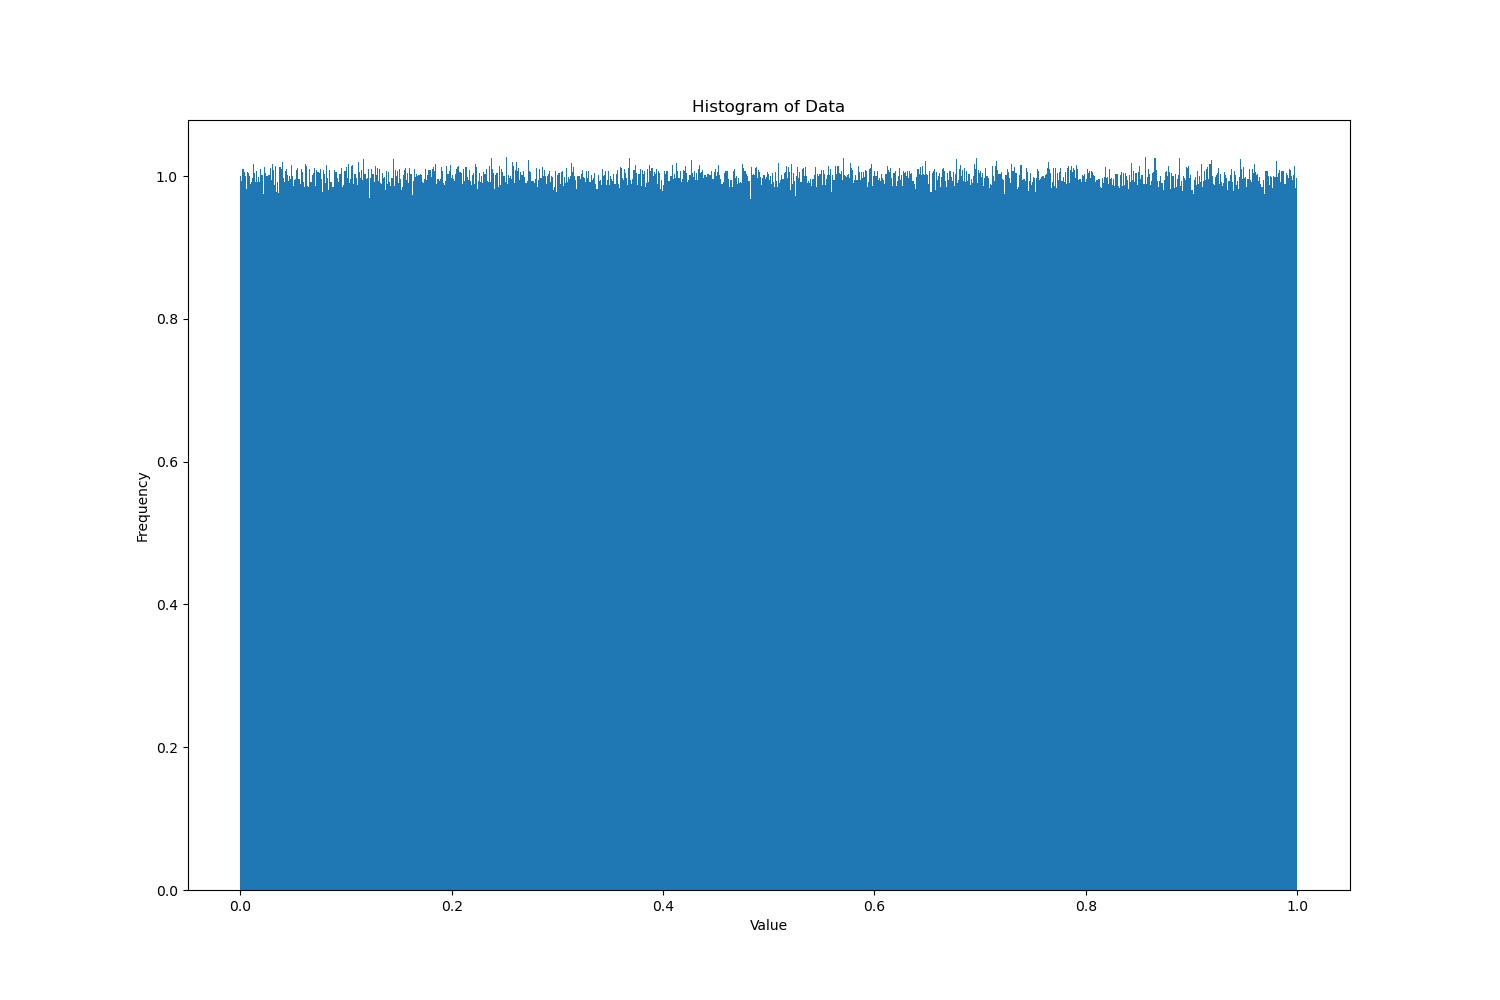
\includegraphics[width=0.32\textwidth]{fig_dist_norm}
			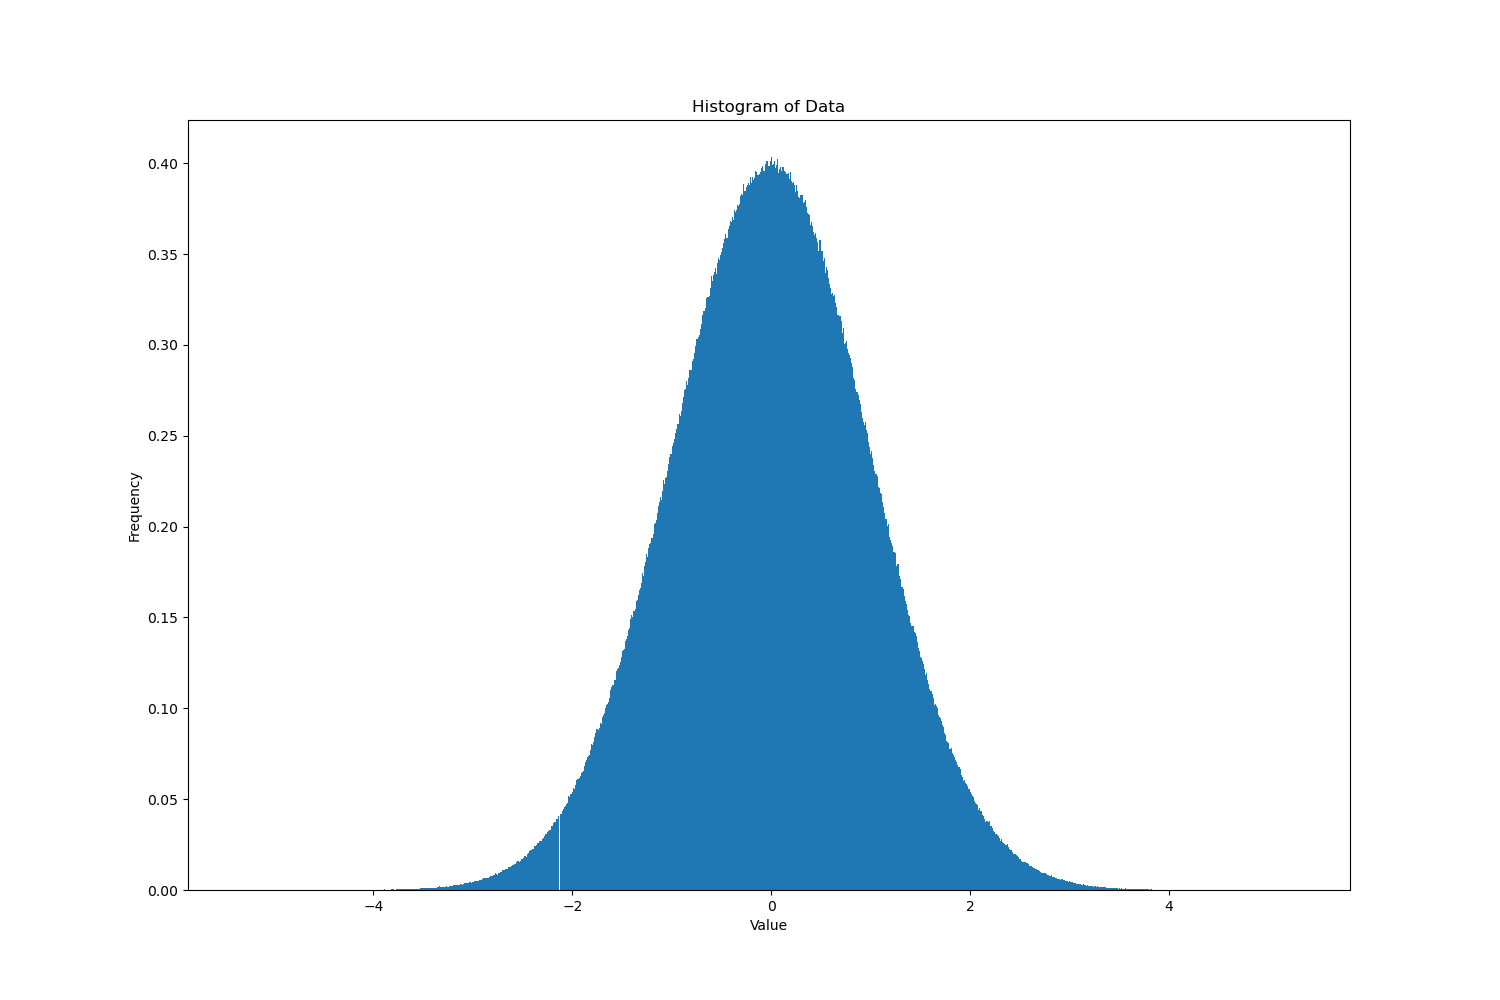
\includegraphics[width=0.32\textwidth]{fig_dist_gauss}
			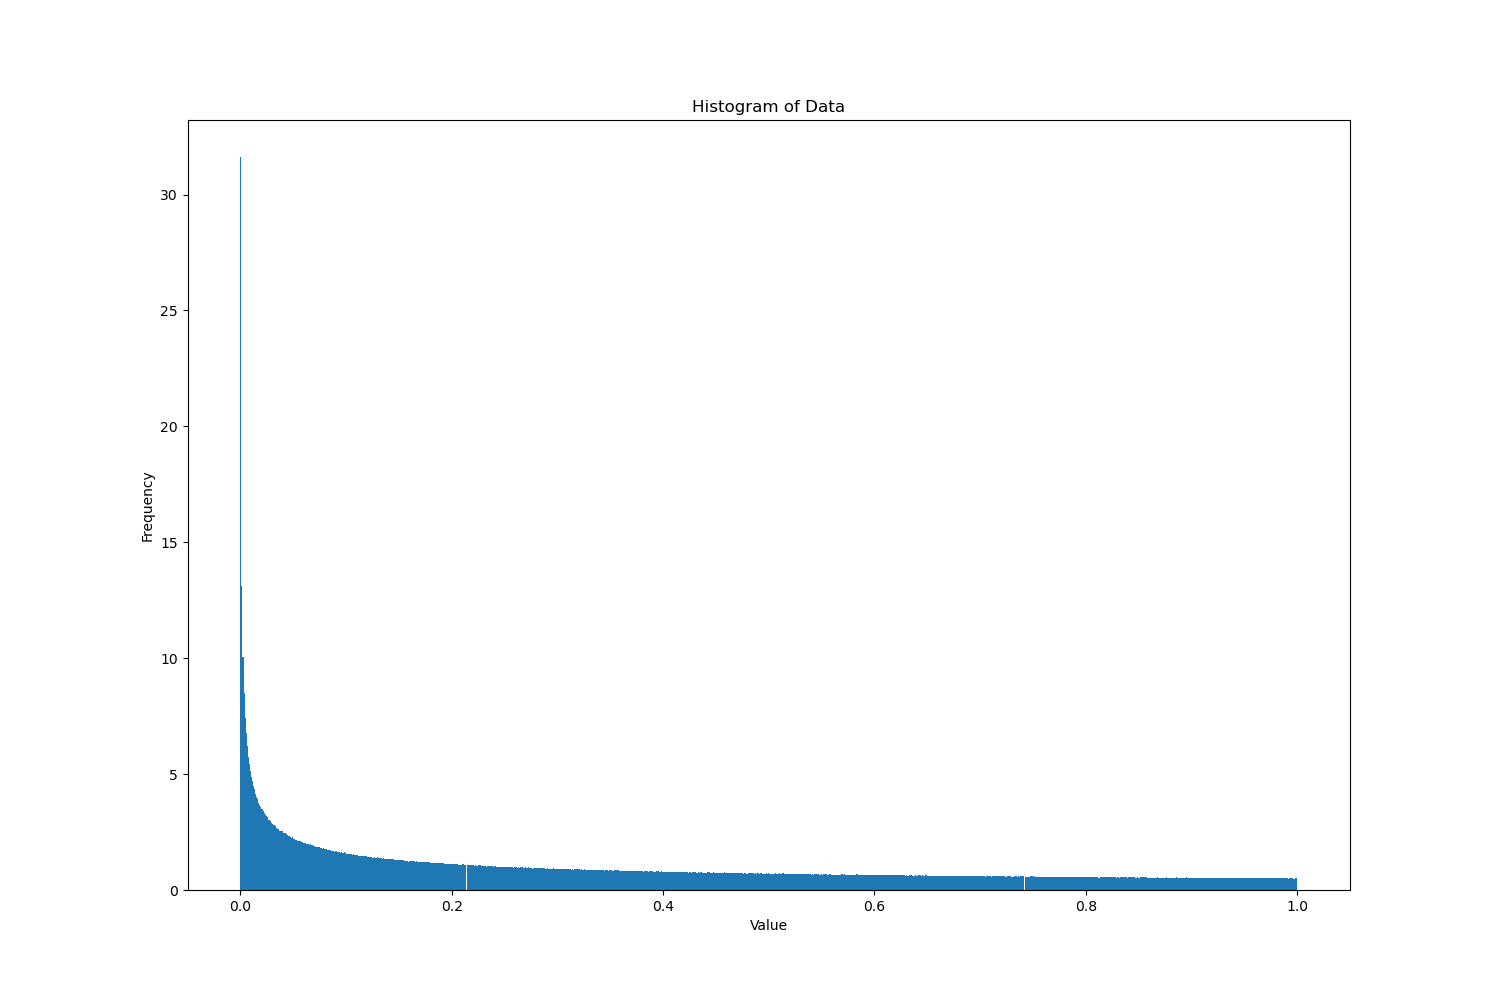
\includegraphics[width=0.32\textwidth]{fig_dist_weird}
		\end{center}
		\caption{Three distributions tested. From left - uniform, Gaussian, and an additional one.}
		\label{fig4}
		\end{figure}		
						
		The reason why statistical sorting is $O(n$) for $n = n_1 n_2$ is because of
		\[
		O(n_1 n_2 \log n_2) \approx O(n_1 n_2) = O(n),
		\]
		as $\log n_2$ is approximately constant for small $n_2$. In case larger $n$ would be measured (over 500000000), it could become again $O(n \log n)$. For our measurements, we can't go over 500000000 due to memory limitations of most linux users (16 GB of RAM memory). 
		As we do recursion in the sorting algorithm, we can show $O(n)$ time complexity as followed:
		\[
		O(n^{1/2} (n^{1/2} \log n^{1/2})),
		\]
		and as $n^{1/2} \log n^{1/2}$ can be sorted again with recursion, we get
		\[
		O(n^{1/2} n^{1/4} (n^{1/4} \log n^{1/4})),
		\]
		and using recursion again and again will get us
		\[
		O(n^{1/2} n^{1/4} n^{1/8} ...) = O(n).
		\]
		So theoretically, using recursion we should get $O(n)$ even for vectors beyond 500000000.
			
		Table \ref{table1} contains selected measurements for time execution and table \ref{table2} contains residuals for determining time complexity of both compared algorithms. These are for uniform distribution, but similar results can be seen for Gaussian distribution in figure \ref{fig2} and an additional distribution in figure \ref{fig3}. All three distributions can be seen in figure \ref{fig4}.
		
		\begin{table}
		\caption{Times for Quick \& Stat Sort for various vector sizes}
		\begin{center}
		\begin{tabular}{ |c|c|c| }
		
		\hline
		
		size & Quick Sort time & Stat Sort time \\

		\hline\hline		
		
		10000		& 1.15760485641658E-08	& 0 \\
		10060050		& 8.27546318760142E-06	& 5.12730912305415E-06 \\
		100510502	& 9.20717575354502E-05	& 5.54861180717126E-05 \\
		201011005	& 0.000190925929928198	& 0.000110023145680316 \\
		301511507	& 0.000290057876554783	& 0.000171666666574311 \\
		402012010	& 0.000397928241000045	& 0.000232824073464144 \\
		500000000	& 0.00049090277752839	& 0.00028194444894325 \\

		\hline
		\end{tabular}
		\end{center}
		\label{table1}
		\end{table}


		\begin{table}
		\caption{Determining time complexity of Quick \& Stat Sort through residuals}
		\begin{center}
		\begin{tabular}{ |c|c|c| }
		\hline
		
		Time complexity & Quick Sort residual & Stat Sort residual \\

		\hline\hline		
		
		$O(n)$ &		27.80140662 &  7.98515784  \\
		$O(n \log n)$ & 13.80724414		& 11.03394399 \\

		\hline
		\end{tabular}
		\end{center}
		\label{table2}
		\end{table}

		
		The entire code for the plots in figure \ref{fig1}, \ref{fig2}, \ref{fig3}, \ref{fig4} and tables \ref{table1} and \ref{table2} can be found on github \cite{peta78}.
		
	\section{Parallelization}
	
	As the initial vector is split into multiple vectors, all the smaller vectors can be sorted in parallel, which makes the statistical sorting algorithm easily parallelizable. As this is quite trivial software engineering work, we will not provide further details in this work, but code for parallelization can be found again on github \cite{peta78b}.

	\section{Discussion \& Future Work}
	
	We introduced statistical sorting and showed from measurements and also by intuition, that its complexity is $O(n)$, which is better than any currently known sorting algorithm on average. On average, all known sorting algorithms have complexity at least $O( n \log n)$. We also compared it with C++ implementation of std sort, which has on average $O(n \log n)$ time complexity. We compared statistical and std sort algorithms on three different vector distributions - uniform, Gaussian and an additional one.
	
	Further work should concentrate on determining best possible threshold for recursion as well what algorithm should be used for sorting tiny vectors (if there is better possibility than C++ std sort). Further work should also look into what happens with vectors of sizes beyond ones measured in this publication as we showed only intuition beyond size of vector 500000000.
	
	\section*{Acknowledgement}
	
	The authors would like to thank Dutch born people of Amsterdam, Netherlands for pleasant working environment in spring of 2023, when idea for statistical sorting was sparked. The authors would like to thank Grammarly for improving English in this work.
	
\begin{thebibliography}{9}
\bibitem{numrec}
Press, William H. and Teukolsky, Saul A. and Vetterling, William T. and Flannery, Brian P. (2007), Numerical Recipes 3rd Edition: The Art of Scientific Computing, Cambridge University Press, USA

\bibitem{gauss}
Carl F. Gauss (1823), Theoria combinationis observationum: erroribus minimis obnoxiae, Gottingae, H. Dieterich, Print

\bibitem{cppsort}
Geek Writers, std::sort() in C++ STL, \url{https://www.geeksforgeeks.org/sort-c-stl/}

\bibitem{wikisort}
Wikipedia Writers, Sorting algorithm, \url{https://en.wikipedia.org/wiki/Sorting_algorithm}

\bibitem{peta78}
Peter Taraba, Statistical sorting algorithm, \url{https://github.com/peta78/Sorting/tree/main/sorting_publication}

\bibitem{peta78b}
Peter Taraba, Statistical sorting algorithm, \url{https://github.com/peta78/Sorting}

\end{thebibliography}

	
	
\end{document}